\chapter{Data Driven Classification of P Cygni and
Inverse P Cygni Spectra with Autoencoders and DTW}

\section{A Brief Recap}

The following conclusions can be drawn from the results presented in the preceding chapters,

\begin{enumerate}
    \item The curse of dimensionality presents a significant challenge when working with high resolution data from million star surveys such as GALAH DR3. 
    \item While popular,  dimensionality reduction techniques such as t-SNE may not be sufficiently robust at identifying emission line spectra. Furthermore, the 2-dimensional t-SNE representation may not be sensitive to the morphological differences between emission line spectra and non-emission line spectra.
    \item Given a data set with emission line spectra, DTW based aggolomerative hierarchical clustering can be used effectively to identify P Cygni and inverse P Cygni spectra.
\end{enumerate}

This chapter builds on these conclusions and presents a proof of concept P Cygni and inverse P Cygni identification pipeline. DTW based agglomerative hierarchical clustering, which  was introduced in chapter 4, forms the basis of this pipeline. Furthermore, this pipeline relies on the pre-selection of H$\alpha$ emission line spectra using an autoencoder first introduced by Čotar et al.

\section{Autoencoders for H$\alpha$ Emission Line Spectra Selection}

Chapter 3 presented an autoencoder neural network that is capable of identifying H$\alpha$ emission line spectra \cite{vcotar2021galah}. This work adapts this approach and exploits it as a pre-processing step prior to the application of DTW based agglomerative hierarchical clustering. The methodology is as follows.

This autoencoder learns the latent space representation of non-emission line spectra but does not learn the latent space representation of emission line spectra accurately. This latent space represents each higher dimensional high resolution spectrum as a 5-dimensional vector. This process is known as encoding. Once the training phase is completed, the autoencoder was fed the total DR3 data set such that it generates predictions for each spectrum. This process is known as decoding. 

The training data is deliberately biased towards non-emission line spectra (so-called normal spectra). Thus for non-emission line spectra, the predicted spectra will match the data more accurately than for emission line spectra. The flux difference between a predicted spectrum and it's observed (original) data counterpart can be exploited to flag emission line stars. This flagging can be accomplished by computing the equivalent width of this "difference spectrum" around the H$\alpha$ line.

\subsection{Autoencoder Architecture and Training}

The autoencoder architecture presented here is similar to the work of Čotar et al. and maps high resolution spectra of dimension 4459 to a 5-dimensional latent space. The popular deep-learning frameworks \texttt{tensorflow}\cite{tensorflow2015-whitepaper} and \texttt{keras}\cite{chollet2015keras} were used to develop the autoencoder.

Each successive dense layer in the neural network reduces the dimensionality of the input layer successively by 75\%, 50\%, 25\% and finally by 10\%. Each layer was activated by the non-linear PReLU function \cite{he2015delving}. The training loss is minimised using the Adam optimiser which performs gradient descent \cite{kingma2014adam}.

\begin{figure}[!htb]
\centering
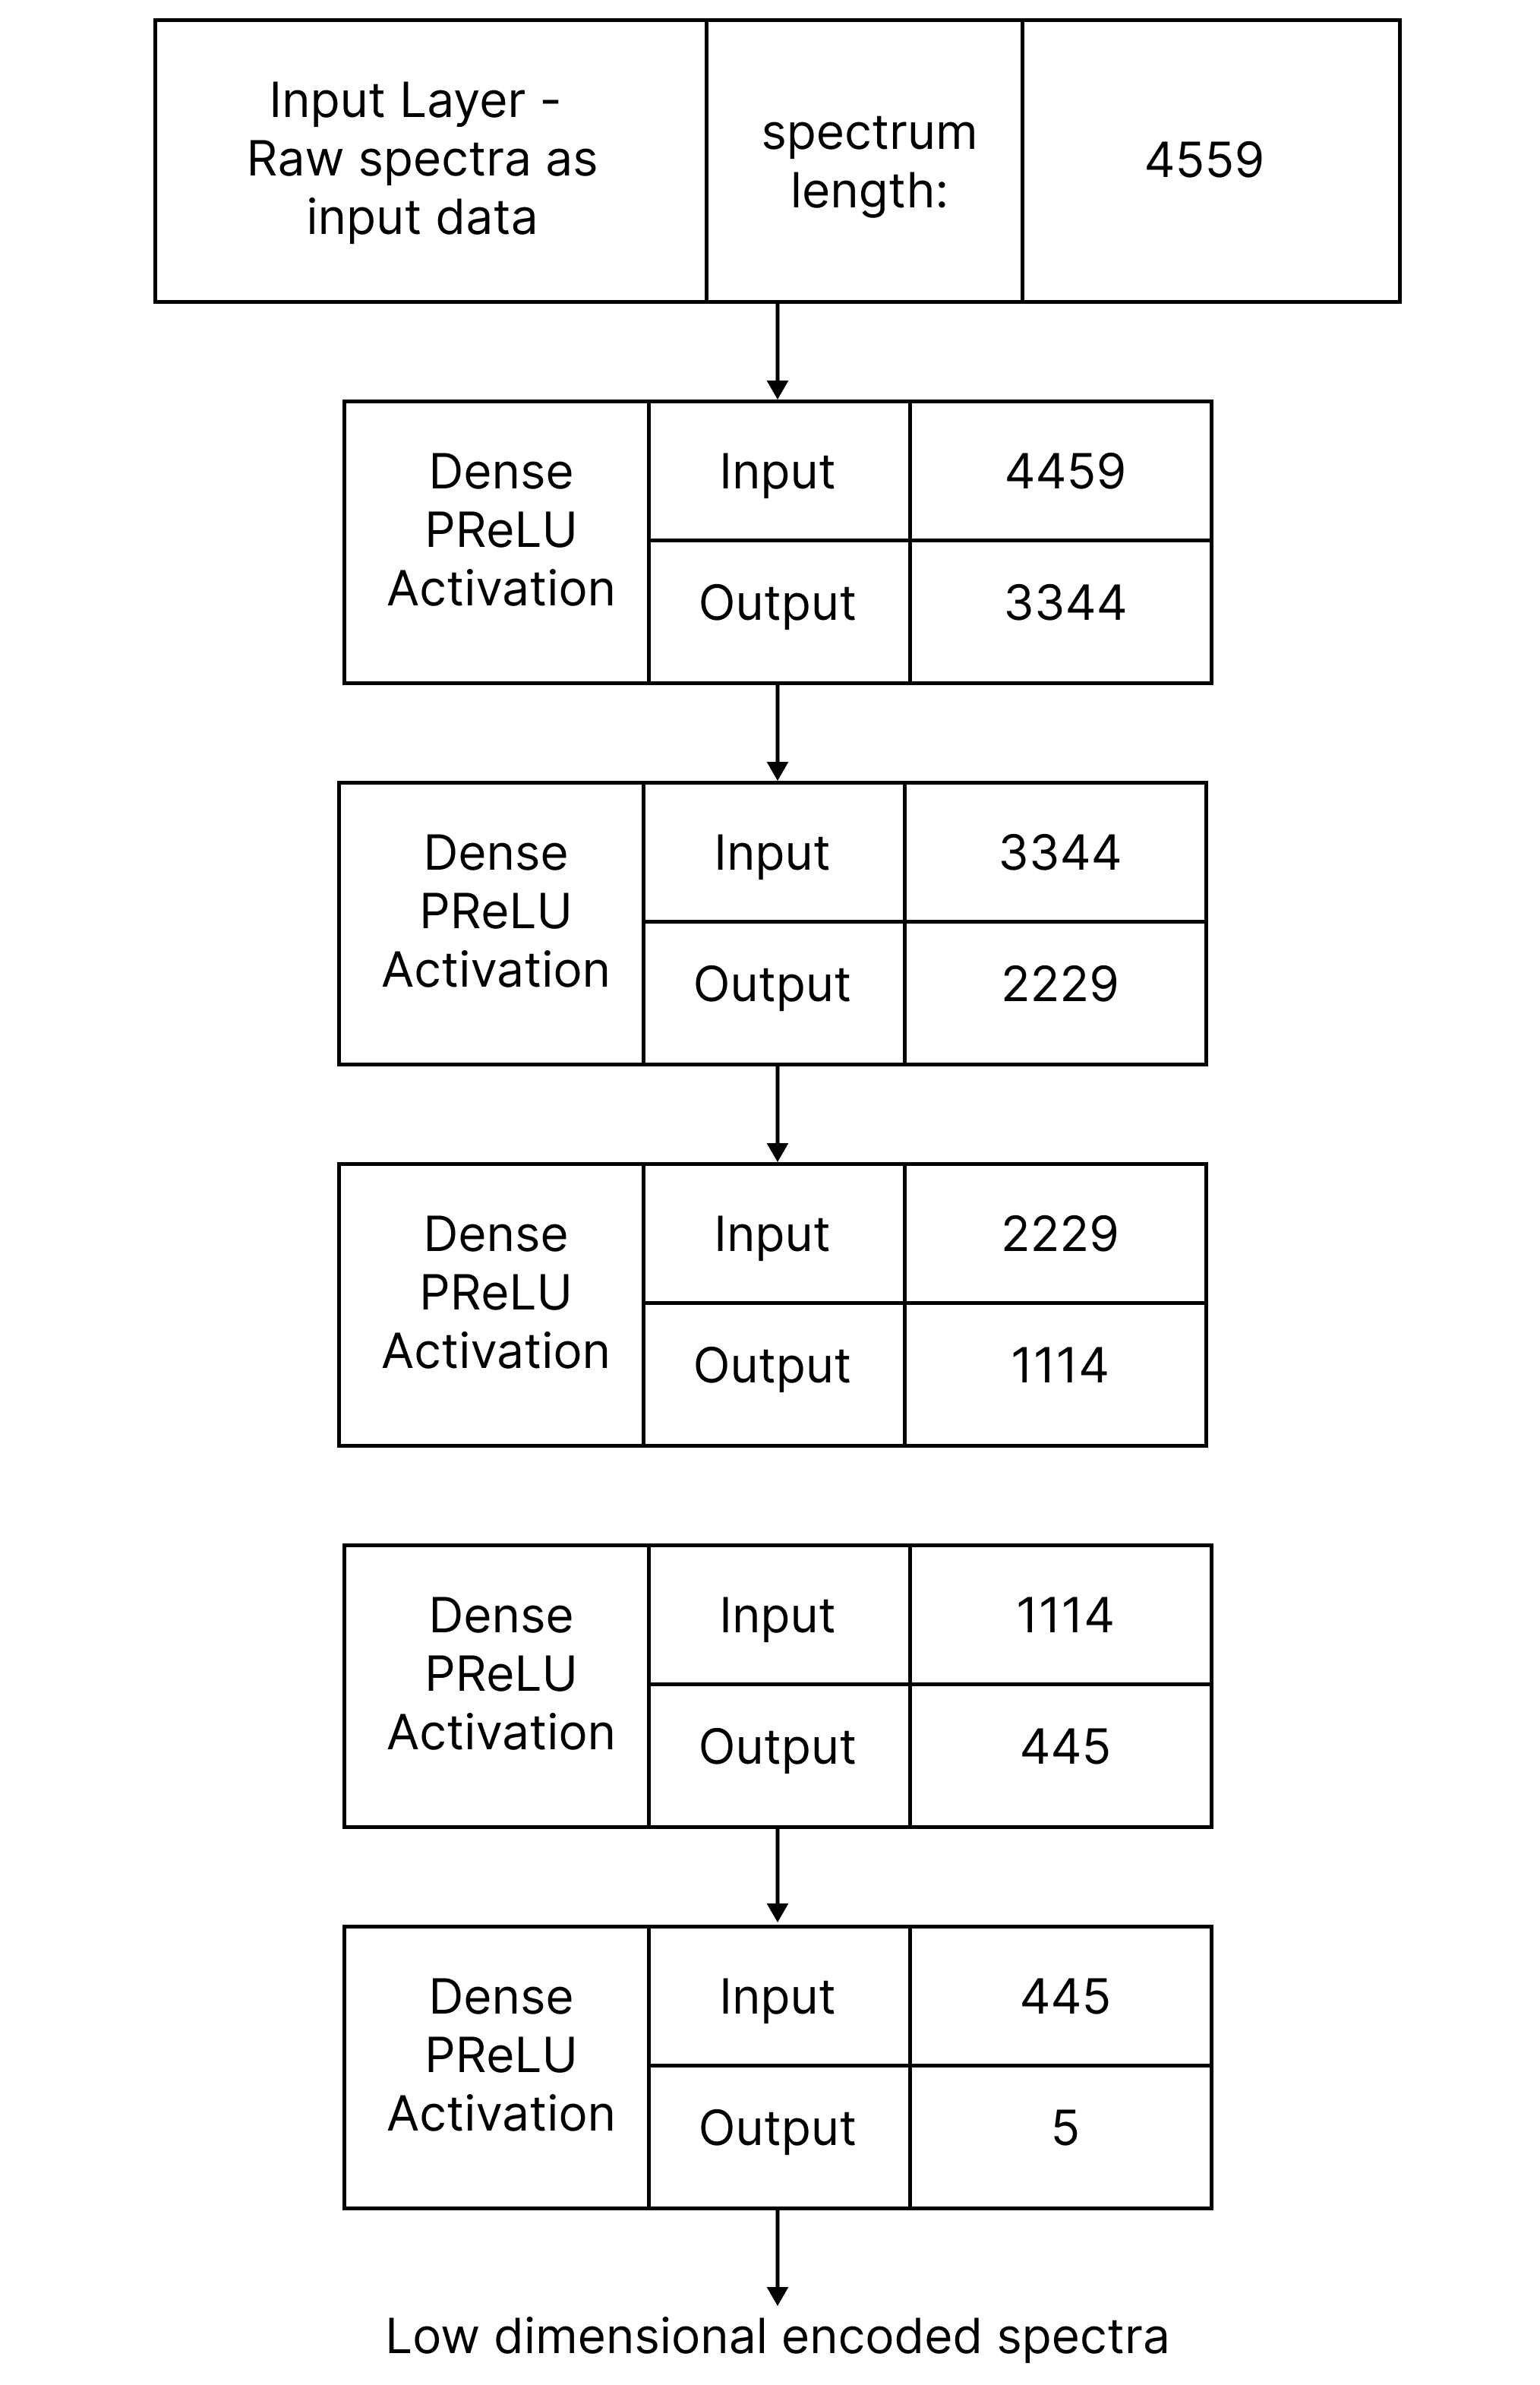
\includegraphics[scale=0.15]{figures/autoencoder diagram.png}
\caption{Visual representation of the encoder. The value in
the right most column indicates the number of input and output
connections to neighboring layers.}
\end{figure}

Čotar et al. recommends inverting the flux values (1 - normalised flux) prior to training and prediction. Greater training stability was achieved by this inversion. Furthermore, they recommend an epoch size of 350 and a batch size of 40,000 spectra. 10\% of the samples were selected as the validation set. This work follows the same conventions. 

For training, the autoencoder requires a training set that's either significantly biased towards non-emission line spectra around H$\alpha$ or contains non-emission line spectra exclusively. In order to select these spectra in DR3, this work uses the quality criteria recommended by Čotar et al.\cite{vcotar2021galah}, Buder et al.\cite{buder2021galah+} and Kos et al.\cite{kos2017galah}. 

While these criteria cannot fully guarantee that the autoencoder will be trained on non-emission line spectra exclusively, prior work by Čotar et al. indicate that they are sufficiently robust for the purpose of training the network. The Data Central SQL/ADQL catalogue query service was used to retrieve GALAH DR3 \texttt{sobject\_id} values that matched these criteria.

\begin{lstlisting}[language=SQL]
SELECT sobject_id
FROM   galah_dr3.main_star
WHERE  snr_c3_iraf > 30
       AND red_flag = 0
       AND flag_sp < 16 
\end{lstlisting}

\begin{table}[!htb]
\begin{center}
\begin{tabular}{|l|l|}
\hline
\textbf{Criterion}    & \textbf{Rationale}                                                                 \\ \hline
SNR \textgreater 30   & Spectra have reduced noise contamination e.g. atmospherics      \\ \hline
\texttt{red\_flag} = 0         & Select spectra that have no know reduction issues                                  \\ \hline
\texttt{flag\_sp} \textless 16 & Select spectra that do not include known emission line spectra identified by t-SNE \\ \hline
\end{tabular}
\caption{Selection criteria for non-emission line spectra for training purposes.}
\label{table:Selection Criteria}
\end{center}
\end{table}

This query returned 396,338 spectra. The red arm data was re-sampled to a common wavelength grid using the methodology outlined in Chapter 2. The normalised flux was then inverted and used as the training data set. The training results are as follows.

\begin{figure}[!htb]
\centering
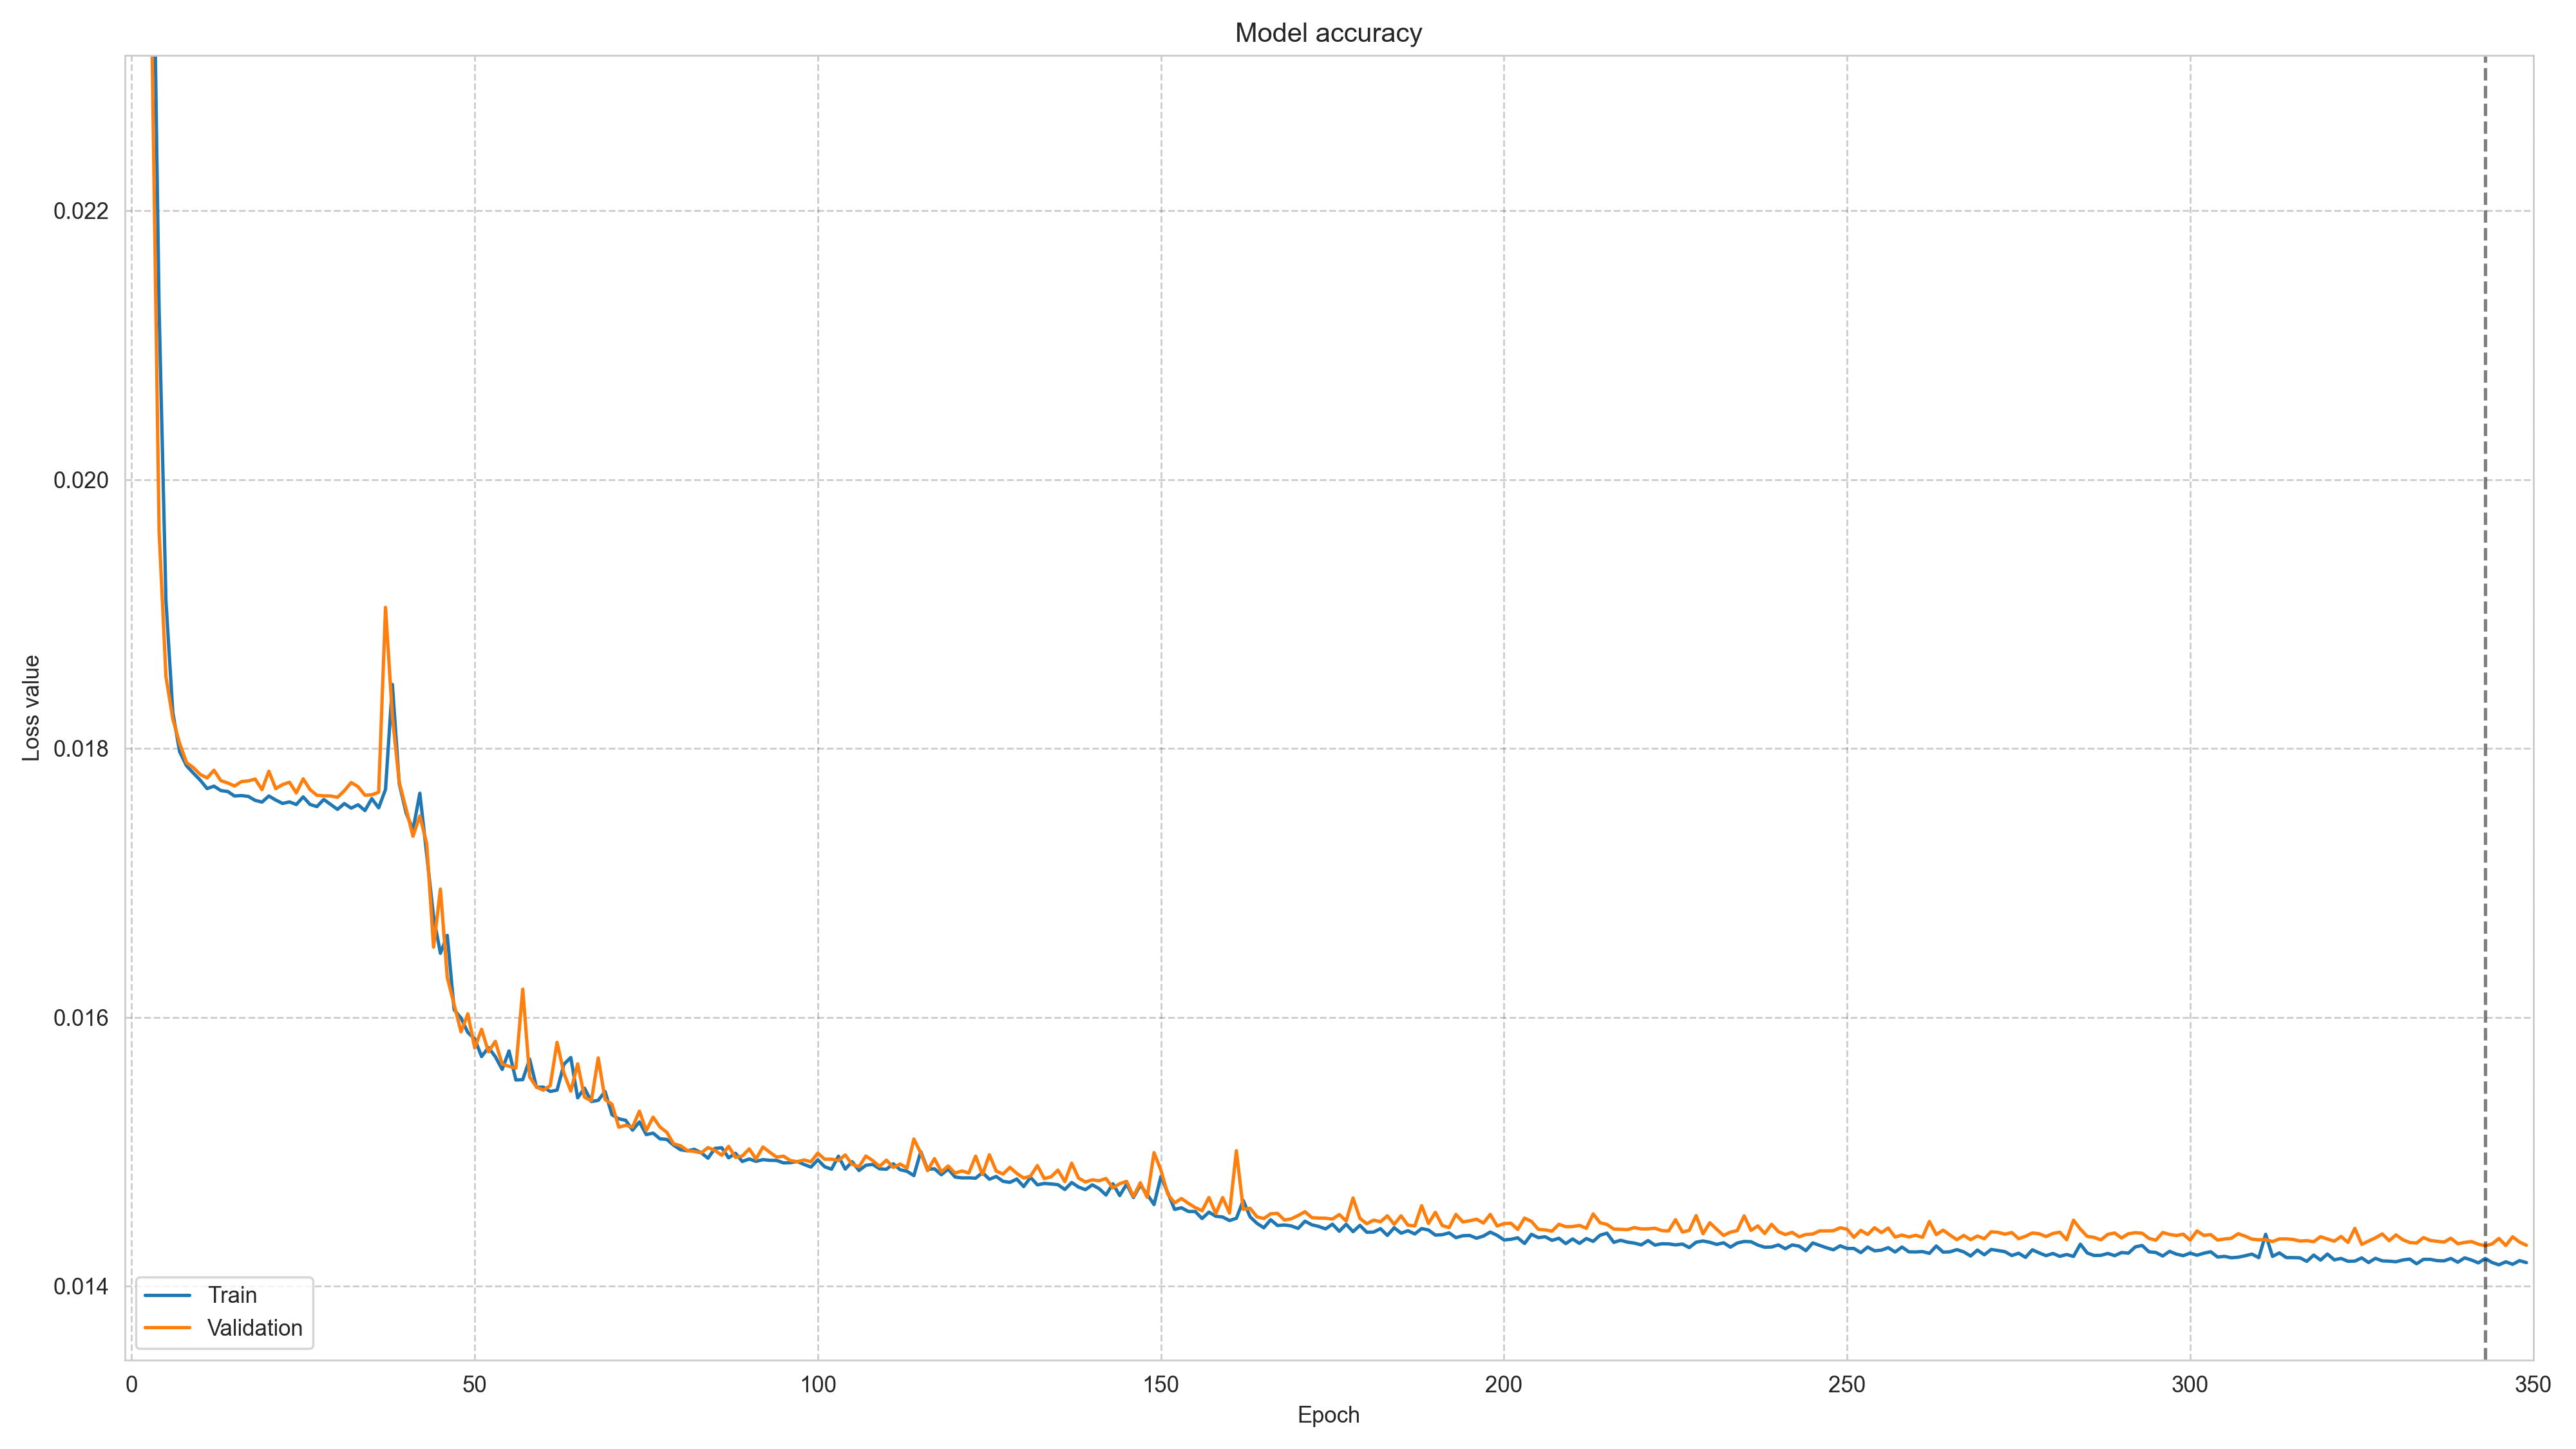
\includegraphics[scale=0.38]{figures/ann_network_loss.png}
\caption{Prediction accuracy of the red arm training dataset at different training epochs.}
\end{figure}

The prediction error for training is computed as a sum of all absolute differences between the input and output data set. Figure 6.2 shows the prediction error of the training process as a function of epoch. At face value, it appears that over-fitting has taken place, however this is a desirable feature in the context of detecting emission line spectra as the network must be sufficiently biased towards non-emission line spectra. Furthermore, these results are in agreement with those presented in Čotar et al.

It is expected that the autoencoder will perform poorly when attempting to reconstruct or predict emission line spectra/fluxes. Conversely, it is expected that it will perform well on emission line spectra. This behaviour has significant implications for the detection of H$\alpha$ emission candidates.

\section{Prediction and Results}

Once the autoencoder was trained, predicted normalised flux of the red arm for each spectrum in DR3 was calculated. Since the input data for training was inverted, all DR3 spectra were inverted prior to input. Thus predicted results from the autoencoder were also inverted.

The difference spectra between the predicted and the original DR3 spectra (observed spectra) were computed. Presented below are the inverted difference spectra for a non-emission line spectrum and a known emission line spectrum in DR3 around H$\alpha$. Note that the non-emission line spectrum produces a difference spectrum with an approximately flat response while the emission line spectrum does not. 

\begin{equation}
   f_{difference} = f_{observed} - f_{predicted}
\end{equation}

\begin{figure}[!htb]
\centering
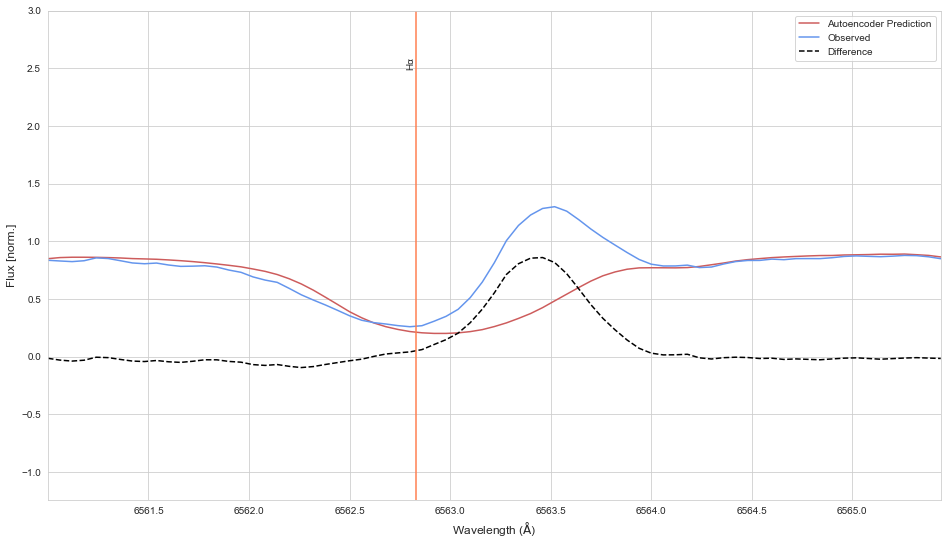
\includegraphics[scale=0.45]{figures/normal difference.png}
\caption{An emission line spectrum (P Cygni), the autoencoder prediction and corresponding difference spectrum. Note the non-flat response of the difference spectrum. This response can be quantified by calculating its equivalent width.}
\end{figure}

\begin{figure}[!htb]
\centering
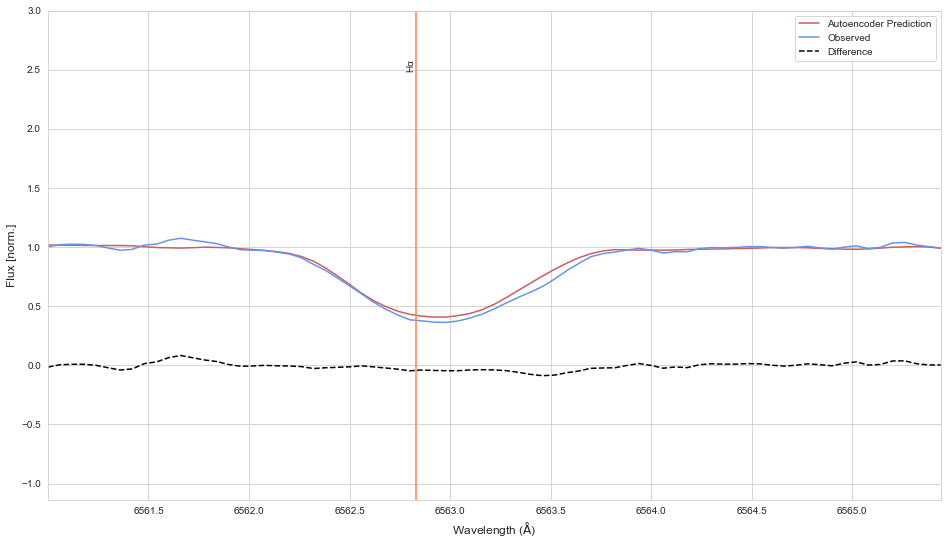
\includegraphics[scale=0.45]{figures/non emission difference.png}
\caption{An non-emission line spectrum, the autoencoder prediction and corresponding difference spectrum. Note the flat response of the difference spectrum. This response can be quantified by calculating its equivalent width.}
\end{figure}

The equivalent width within the range 6561\r{A} - 6565\r{A} was determined using the popular Python packages \texttt{astropy}\cite{astropy:2018}\cite{astropy:2013} and \texttt{specutils}\cite{specutils}. For consistency, these widths were calculated for the inverted difference spectra. Čotar et al. used an equivalent width cut-off of 0.25 to separate emission line spectra from DR3. This work follows the same approach. The histogram of equivalent widths of the 6,093 spectra thus obtained was examined and was in agreement with the results from Čotar et al. 

\begin{figure}[!htb]
\centering
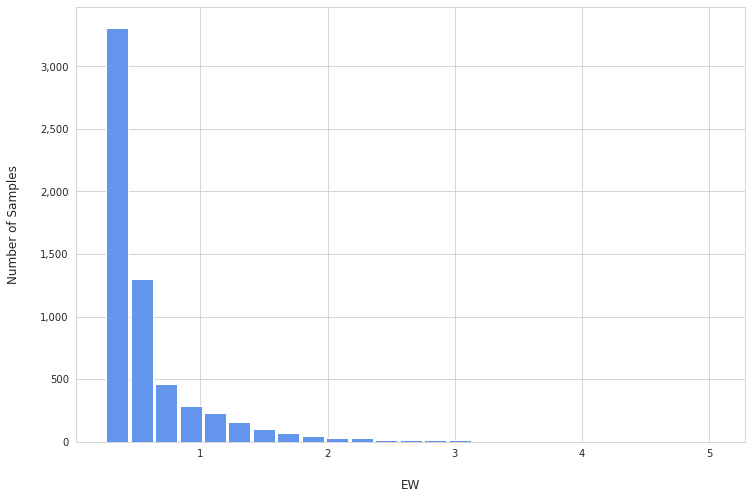
\includegraphics[scale=0.45]{figures/EW hist.png}
\caption{The equivalent width (EW) distribution of the inverted difference spectra of the emission line candidates identified by the autoencoder. Here EW > 0.25.}
\end{figure}

\section{DTW Based Agglomerative Hierarchical Clustering}

The next step in the analysis pipeline is identical to the methodology introduced in Chapter 4. DTW distances were calculated for the emission line spectra and agglomerative hierarchical clustering was used to 

